%\documentclass[journal=jctcce,manuscript=article]{achemso}
\documentclass[11pt,oneside,a4paper]{article}
\usepackage[T1]{fontenc}
\usepackage{graphicx}
\usepackage{amsmath,amssymb,mathrsfs}
%\usepackage{xr}
\usepackage{booktabs}
\usepackage{multirow}
\usepackage{siunitx}
\usepackage{easy-todo}
%\usepackage{footref}
%\externaldocument[S-]{SI}

\sisetup{
  separate-uncertainty = true
}

\renewcommand{\footnoterule}{}
\renewcommand{\vec}[1]{\mathbf{#1}}


\title{Charging free energy corrections}

%\input{affiliations}

%\keywords{Free Energy, Hydration, Alchemical, Reproducibility, Automation}



\begin{document}

%\begin{abstract}

%\end{abstract}


%\section{Introduction}
%\label{sec:intro}


\section{Methods}
\label{sec:methods}

\subsection{Dataset and molecules parametrization}
\label{sec:parametrization}

\todo{Add image of the CBC Datasetand CBC (SAMPL5 paper HG)}

For the 2015 Statistical Assessment of Modelling Proteins and Ligands (SAMPL5) blind free energy predictions for a dataset of host-guest systems were requested from all the participants. Figure XX shows one of the three SAMPL5 datasets, which consists of 10 charged guests that binds to a cucurbituril clip (CBC) at a physiological pH (7.4).
The CBC is flexible host, which has shown a high binding affinity to ferrocene, adamantane and bicyclooctane guests $\cite{CBC_1,CBC_2,Grimme2014}$. Experimental data for CBC host-guest complexes were obtained using UV, visible and fluorescent spectroscopic measurements. All data were measured in the laboratory of Bruce Gibb (Tulane University) ~\cite{yin2016overview}.

Both host and guest were parametrized with AM1-BCC charges and general Amber force field (GAFF).
Initially, guest free phase topology and coordinates files were created by using the protocol described in ~\cite{bosisio2016blinded}. Guest force field parameters were extracted from bound phase files.  Thus, guests were solvated in a rectangular box of TIP3P water molecules $\cite{Jorgensen1983}$ with a minimum distance between solute and box surface of 12 $\AA$, using \textit{tleap}. Ions were added to neutralize the overall charge of the box. The system was energy minimized with 100 steps of steepest descent algorithm. Then, solute's atoms were position restrained with a force constant of \SI{10}{kcal mol^{-1}\AA^{-2}}, to allow water to equilibrate in an NVT ensemble for \SI{200}{ps} at \SI{298}{K}, followed by an NPT equilibration for further \SI{200}{ps} at \SI{1}{atm} pressure, with Amber module Sander ~\cite{AMBER}. Lastly, \SI{2}{ns} of NPT simulation were run with Sire/SOMD (rev 15.1)~\cite{Sire,OpenMM} and a final coordinate file was extracted from the last trajectory snapshot with CCPTRAJ~\cite{CPPTRAJ}. This protocol will be called ``SAMPL5 box'' through the paper.
Recently, a second protocol, ``iso box'' protocol, was adopted to create guest files in solvated phased. In particular, host heavy atoms were substituted with water molecules. Thus, a minimization on the system was performed along with the equilibration steps described above. In this way, the final solvated phase box dimensions were equal to the bound phase ones, avoiding further box size effects problems. 


\subsection{Alchemical binding free energy}
\label{sec:freeenergy}
\todo{add picture for the TD cycle double annihilation}
Binding free energies $\Delta G_{\mathrm{bind}}$ were estimated from MD simulations by means of a double annihilation technique proposed originally by Jorgensen et al.$\cite{Jorgensen1988}$ and developed by Gilson et al.$\cite{Gilson1997}$. As depicted in fig XX $\Delta G_{\mathrm{bind}}$ can be estimated as:
\begin{equation}
 \label{eq:dgbind}
 \Delta G_{\mathrm{bind}} = -k_{\mathrm{B}}T \ln \frac{Z_{\mathrm{HG,solv}} Z_{\mathrm{solv}}} {Z_{\mathrm{G,solv}} Z_{\mathrm{H,solv}} }
\end{equation}
where $k_{\mathrm{B}}$ is the Boltzmann constant, $T$ the temperature, $Z_{\mathrm{HG,solv}}$, $Z_{\mathrm{G,solv}}$, $Z_{\mathrm{H,solv}}$,$Z_{\mathrm{solv}}$ are the configuration integrals for host-guest complex, the guest, the host and the solvent molecules respectively. Figure XX depicts how the double annihilation approach may be used to evaluate $\Delta G_{\mathrm{bind}}$ employing a thermodynamic cycle. First the guest's partial charges are turned off both in water and in the host-guest-complex phase (discharging step), giving the discharging free energy change $\Delta G_{\mathrm{elec}}^{\mathrm{solv}}$ and $\Delta G_{\mathrm{elec}}^{\mathrm{host}}$ respectively. Secondly, the guest is fully decoupled from the solvent or host, switching off the van der Waals terms (vanishing step), $\Delta G_{\mathrm{vdW}}^{\mathrm{solv}}$ and $\Delta G_{\mathrm{vdW}}^{\mathrm{host}}$. The discharging and vanishing steps are usually performed with a series of intermediate simulations that depend on a coupling parameter $\lambda \in [0,1]$. Closure of the thermodynamic cycle gives the free energy of binding $\Delta G_{\mathrm{bind}}$ as$\cite{Michel2010}$:
\begin{equation}
 \label{eq:annihilation}
 \Delta G_{\mathrm{bind}} = ( \Delta G_{\mathrm{elec}}^{\mathrm{solv}} + \Delta G_{\mathrm{vdW}}^{\mathrm{solv}} ) -
 (\Delta G_{\mathrm{elec}}^{\mathrm{host}} + \Delta G_{\mathrm{vdW}}^{\mathrm{host}} )
\end{equation}

In the actual MD simulation an empirical distance-restraint term is added to the potential energy function. This is done to prevent the non-interacting guest from drifting out of the host cavity. A flat-bottom restraining potential is used between one atom of the guest, chosen to be the one closest to the centre of mass, and four equivalent carbon atoms of the host. The restraint potential for atom $j$ of the guest is based on work by Michel et al.$\cite{Michel2014}$:
\begin{equation}
 \label{eq:restraint}
 U^{\mathrm{restr}}(d_{j1},...,d_{jN_host}) = \sum_{i=1}^{N_{\mathrm{host}}}
\begin{cases}
0  & if |d_{ji} - R{ji}| \le D_{ji}\\
\kappa_{\mathrm{ji}} (|d_{ji} -R_{ji}| - D_{ji} )^2  & if |d_{ji} - R_{ji}| > D_{ji}
\end{cases}
\end{equation}
where $U^{\mathrm{restr}}(d_{j1},...,d_{jN_{host}})$ is the potential energy of the restraint as a function of the distance between a guest atom $j$ and a set of host atoms $i$, $d_{ji}$=$|| \mathbf{r_{\mathrm{i}}} - \mathbf{r_{\mathrm{j}}} ||$, $D_{\mathrm{ji}}$ is the restraint deviation tolerance, $R_{\mathrm{ji}}$ the reference distance between host and guest atom, $\kappa$ the restraint force constant and $N_{\mathrm{host}}$ the number of host atoms that contribute to the restraint. Introduction of the flat-bottom restraint brings to the calculation of a restraint free energy change  $\Delta G^{\circ}_{\mathrm{restr}}$, as fig XX shows, computed as:
\begin{equation}
 \label{eq:DGrestr}
 \Delta G_{\mathrm{restr}}^{\circ} = -k_{\mathrm{B}}T\ln \left ( \frac{Z_{\mathrm{H\bullet\bullet G^{\mathrm{ideal}},solv}} }{Z_{\mathrm{H,solv}}Z_{\mathrm{G,gas}}} \right )
\end{equation}
where $Z_{\mathrm{H\bullet\bullet G^{\mathrm{ideal}}, solv}}$ is the configuration integral for the restrained decoupled guest bound to the host, $Z_{\mathrm{H,solv}}$ is the configuration integral for the solvated host and $Z_{\mathrm{G,gas}}$ for the guest in an ideal thermodynamic state. Assuming that the restraint potential is decoupled form the solvent and host degrees of freedom, eq~\ref{eq:DGrestr} simplifies to:
\begin{equation}
 \label{eq:DGrestrcomp}
 \Delta G_{\mathrm{restr}}^{\circ} = -k_{\mathrm{B}}T\ln \left (
 \frac{Z_{\mathrm{\bullet\bullet G^{\mathrm{ideal}},solv}}}{Z_\mathrm{G,gas}}
 \right )
\end{equation}
where $Z_{\mathrm{\bullet\bullet G^{\mathrm{ideal}},solv}}$ is the configuration integral for the decoupled guest. Because the guest  has no intermolecular interactions in both thermodynamic states defined in eq.~\ref{eq:DGrestrcomp}, and because the restraint does not hinder rotational motions, internal and rotational contributions cancels cancels out and the only term left is the translational contribution to the configuration integral. For $Z_{\mathrm{G,gas}}$ a standard volume of measurement $V^\circ$ is used, with the \SI{1}{M} dilute solution convention $V^\circ$=\SI{1660}{\AA^3 mol^{-1}}. Therefore eq.~\ref{eq:DGrestrcomp} simplifies further to:
\begin{equation}
\label{eq:DGrestr2}
\Delta G_{\mathrm{restr}}^\circ = -k_{\mathrm{B}}T\ln \left ( \frac{ V^\mathrm{restr}}{V^\circ} \right )
\end{equation}
where the restraint volume $V^\mathrm{restr}$ is :
\begin{equation}
 \label{eq:vrestr}
 V^\mathrm{restr}= \int_{-\infty}^{+\infty}
 \int_{-\infty}^{+\infty}
 \int_{-\infty}^{+\infty}
 dx_jdy_jd_zj exp(-\beta U^\mathrm{restr}(d_\mathrm{j1},...,d_\mathrm{jN_{host}}))
\end{equation}
$V^\mathrm{restr}$ can be calculated numerically: first, the coordinates of the host-guest complex in the generate trajectory at $\lambda$=1 of the vanishing step were aligned to the first frame of the trajectory. Then, the average coordinates of each of the four host atoms used for the restraint were computed. Next, a grid of \SI{0.1}{\AA} and  a rectangular cuboid given by the minimum/maximum coordinates of the four host atoms were defined.
Thus, numerical integration was performed via multidimensional trapezoidal rule.
By subtracting $\Delta G_{\mathrm{rest}}^\circ$ to eq. ~\ref{eq:dgbind} the standard free energy of binding is computed.

\subsection{Poisson-Boltzmann equation for charging free energy corrections}
\label{sec:pbcorrection}

Corrections for discharging free energy were taken into consideration to estimate the final standard free energy of binding $\Delta G_{\mathrm{bind}}^\circ$. These corrections are based on the seminal works by Reif and Oostenbrink $\cite{Reif2014}$, Rocklin et al. $\cite{Rocklin}$ and earlier papers from Kastenholz and H{\"u}nenberger $\cite{Kastenholz1,Kastenholz2}$. Here corrections for free energy estimation were tuned for a Barker Watts Reaction field $\cite{BWRF}$ with atom based cutoff.
First, periodic boundary conditions (PBC), box size effects and polarization issues were treated.
PBC allows to approximate an infinite real system by using a small part of it, the unit cell. In this way simulations can be computationally efficient, but a deviation from real system polarization may be introduced.
Box size effects have been documented by Kastenholz and H{\"u}nenberger$\cite{Kastenholz1,Kastenholz2}$ and Rocklin$\cite{Rocklin}$ and can introduce a bias up to \SI{20}{kcal.mol^{-1}} for charged systems.
Polarization issues arises mainly for the effective Coulombic potential employed. Furthermore, solvent model may have a dielectric constant different from the real solvent, introducing bias in polarization around the charged solute.
To correct these three sources of errors a correction term $\Delta G_{\mathrm{POL}}$ was computed as:
\begin{equation}
 \label{eq:DGPOL}
 \Delta G_\mathrm{POL} = \Delta G_\mathrm{NP}^\mathrm{Coul} -
			\Delta G_\mathrm{RF}^\mathrm{Coul}
\end{equation}
where $\Delta G_\mathrm{NP}^{\mathrm{Coul}}$ is the electrostatic charging free energy due to Coulombic interactions under non-periodic conditions. $\Delta G_\mathrm{RF}^\mathrm{Coul}$ is the electrostatic charging free energy obtained solving the Poisson equation under BWRF and periodic boundary conditions, using a custom code kindly given us by H{\"u}nenberger $\cite{peter2003fast}$.
In particular, $\Delta G_\mathrm{NP}^\mathrm{Coul}$ is computed by using \textit{APBS} software ~\cite{APBS}. First, the trajectory file is loaded and all the snapshots are aligned onto the first one. Secondly, 193 grid points per processor are selected for grid creation with a mesh-grid spacing of \SI{0.50}{\AA}. Thus, \textit{APBS} performs a non periodic electrostatic potential calculation on the host-guest system retrieving the potential $\phi^\mathrm{HG}(\mathbf{r})$ as a function of coordinates $\mathbf{r}$. From this potential an electrostatic free energy change $\Delta G_\mathrm{NP}^\mathrm{HG}$ can be evaluted as:
\begin{equation}
 \label{eq:DGNPHG}
 \Delta G_\mathrm{NP}^\mathrm{HG} = \sum_{i=1}^{N_\mathrm{solute}} q_\mathrm{i}\phi^\mathrm{HG}(\mathbf{r_\mathrm{i}})
\end{equation}
where the sum is extended to all the solute's atoms $N_\mathrm{solute}$, $q_\mathrm{i}$ is the $i$-th solute atom charge and $\phi^\mathrm{HG}(\mathbf{r_\mathrm{i}})$ is the electrostatic potential $\phi^\mathrm{HG}(\mathbf{r})$ at the $i$-th site.
Then, the same grid is used  to evaluate an electrostatic potential $\phi^\mathrm{H}(\mathbf{r})$ setting the guest's charges to zero, obtaining a $\Delta G_\mathrm{NP}^\mathrm{H}$ using eq~\ref{eq:DGNPHG} with $\phi^\mathrm{H}(\mathbf{r})$.
As described in ~\cite{gilson1993computation,madura1995electrostatics,fogolari2002poisson} for each electrostatic potential calculation a vacuum reference potential is evaluated, in order to cancel out the self the Coulombic terms.
The final electrostatic charging free energy $\Delta G_\mathrm{NP}^\mathrm{Coul}$ is computed as a difference:
\begin{equation}
 \label{eq:DGNPcoul}
 \Delta G_\mathrm{NP}^\mathrm{Coul} = \Delta G_\mathrm{NP}^\mathrm{HG} - \Delta G_\mathrm{NP}^\mathrm{H}
\end{equation}


Secondly, the presence of an atom-based cutoff introduces errors in computing solute-solvent interactions. This summation scheme causes an apparent solvation of negatively charged species and a de-solvation of positively charged molecules. For atom-based BWRF a $\Delta G_\mathrm{PSUM}$ correction term was evaluated as:
\begin{equation}
 \label{eq:DGPSUM}
 \Delta G_\mathrm{PSUM} = -\frac{N_A}{6\epsilon_0} Q_\mathrm{mol}\gamma_s \left[ \left( \frac{2(\epsilon_\mathrm{BW} + 1)}{2\epsilon_\mathrm{BW} +1 } \times \frac{\langle N_\mathrm{s}(r_\mathrm{c}) \rangle} {4\pi \frac{r_c^3}{3} } \right) + \frac{3}{2\epsilon_\mathrm{BW} +1 } \right]
\end{equation}
where $N_A$ is Avogadro number, $\epsilon_0$ the experimental permittivity for the solvent, $\epsilon_\mathrm{BW}$ the dielectric constant of the water model used, $\gamma_s=\sum_\mathrm{i=1}^\mathrm{N} q_\mathrm{i}\mathbf{r_\mathrm{i}}$ is the trace of the quadrupole-moment tensor of the solvent model, where the sum is over all $N$ atoms in a solvent molecule, $q_\mathrm{i}$ is the charge of the $i$-th atom in a solvent molecule, $\mathbf{r_\mathrm{i}}$ is the coordinate vector, $Q_\mathrm{mol}$ is the net charge of the solute,$r_\mathrm{c}$ is the reaction field cutoff length and $\langle N_\mathrm{s}(r_\mathrm{c})\rangle$ the average number of solvent molecules within $r_\mathrm{c}$. $\langle N_\mathrm{s}(r_\mathrm{c})\rangle$ was evaluated considering the distance between solutes'atoms and the centre of mass of each water molecule.

Finally, employing an effective Coulombic potential gives a bias in the guest-host interactions. Thus a $\Delta G_\mathrm{dir}$ term was computed as:
\begin{equation}
 \label{eq:DGDIR}
 \Delta G_\mathrm{dir} = U_\mathrm{NP}^\mathrm{dir} - U_\mathrm{RF}^\mathrm{dir}
\end{equation}
where $U_\mathrm{NP}^\mathrm{dir}$ is the sum of the intermolecular and intramolecular solute energies under Coulomb's law and $U_\mathrm{RF}^\mathrm{dir}$ is the sum of intermolecular and intramolecular solute energies with BWRF Coulombic potential.

The final charging correction term is:
\begin{equation}
 \label{eq:DGCOR}
 \Delta G_\mathrm{COR}= (\Delta G_\mathrm{NP}^\mathrm{HG} + \Delta G_\mathrm{NP}^\mathrm{H} + U_\mathrm{NP}^\mathrm{dir} ) - (\Delta G_\mathrm{RF}^\mathrm{HG} + \Delta G_\mathrm{RF}^\mathrm{H} + U_\mathrm{RF}^\mathrm{dir} ) 
\end{equation}
giving a final standard free energy of binding $\Delta G_\mathrm{bind}^{\circ}$ :
\begin{equation}
 \label{eq:DGBINDCOR}
 \Delta G_\mathrm{cor}^\circ= \Delta G_\mathrm{bind} + \Delta G_\mathrm{restr}^\circ + \Delta G_\mathrm{COR}^\mathrm{PBcode}
\end{equation}


\subsection{A termodynamic cycle for charging free energy corrections}
\label{sec:tdcorrection}

To have a comparison term and assess the magnitude of the charging free energy corrections computed as described in ~\ref{sec:pbcorrection}, a thermodynamic cycle approach was tested, too. As depicted in fig XX, in order to maintain the electroneutrality at the beginning and at the end of each leg of the thermodynamic cycle as many dummy counterions as the charge of the solute can be added to the box. Thus, once the solute is fully decoupled, van der Waals parameters and charge of each ion are sequentially switched on both in solvated and bound phases. In this way, considering $n$ counterions, a correction term $\Delta G_\mathrm{COR}^\mathrm{ion}$ can be computed as:
\begin{equation}
 \label{eq:DGCORion}
 \Delta G_\mathrm{COR}^\mathrm{TDion} =\sum_\mathrm{i=1}^\mathrm{n} \left\{ \Delta G_\mathrm{ion_i}^\mathrm{solv} - \Delta G_\mathrm{ion_i}^\mathrm{host} \right\}% \sum_\mathrm{i=1}^\mathrm{n} \left\{ (\Delta G_\mathrm{ion_i elec}^\mathrm{solv} ) + \Delta G_\mathrm{ion_i vdW}^\mathrm{solv} ) - (\Delta 
 %G_\mathrm{ion_i elec}^\mathrm{host} + \Delta G_\mathrm{ion_i vdW}^\mathrm{host} ) \right\} = 
\end{equation}
where the sum is extended up to all the $n$ counterions,
$\Delta G_\mathrm{ion_i}^\mathrm{solv}$ is the free energy change for turning on van der Waals and charges of the $i$-th ion in the solvated phase, $\Delta G_\mathrm{ion_i}^\mathrm{host}$ is the free energy change for the $i$-th ions in the bound phase.


\subsection{Alchemical free energy production simulations}
\label{sec:afesim}

For the discharging step nine equidistant $\lambda$ windows were selected for the host-guest complex and the guest in water phase. Differently, for the vanishing step eighteen equidistant windows were employed, in order to guarantee good overlap of the potential energy distributions of neighbouring $\lambda$ windows.
Initially, for the SAMPL5 challange all the host-guest systems were run for \SI{16}{ns} with a velocity-Verlet integrator timestep of \SI{4}{fs} using a hydrogen mass repartitioning (HMR) scheme ~\cite{hopkins2015long}. For more recent simulations, HMR was not adopted, once convergence tests were made to assure the same results were attained. All simulations were performed in an NPT ensemble and temperature control was achieved with an Andersen Thermostat with a coupling constant of \SI{10}{ps^{-1}}~\cite{Thermostat}. Pressure was manintained by a Monte Carlo barostat, attempting isotropic box edge scaling every \SI{100}{fs}. Periodic boundary conditions were imposed with a \SI{12}{\AA} atom-based cutoff distance for the non-bonded interactions, using a Barker Watts reaction field with a dielectric constant of 82.0~\cite{BWRF}. In the host-guest complex the molecules were restrained according to eq.~\ref{eq:restraint}. The parameters were $R_\mathrm{ji}$=\SI{5}{\AA} , $D_\mathrm{ji}$=\SI{2}{\AA} and $\kappa_\mathrm{ji}$=\SI{10}{kcal mol^{-1} \AA^{-2} }.
Individual free energy contributions from the discharging and vanishing steps were estimated by using MBAR~\cite{MBAR}. To estimate the accuracy and consistency of the computed binding free energy, each simulation was repeated twice using different initial assignments of velocities drawn from the Maxwell-Boltzmann distribution. Final binding free energies are reported as average of both runs and statistical uncertainties were calculated according to:
\begin{equation}
 \label{eq:stderr}
err(\Delta G) = \frac{\sigma}{\sqrt{n}}
\end{equation}
where $\sigma$ is the standard deviation of both runs and $n$=2.

The computed binding free energies are then compared to experimental values considering the determination coefficient $R^2$ and the mean unsigned error MUE. To gain insight into the distribution of the two differnet measures a bootstrapping scheme is used in which each computed free energy point is considered to parametrize a normal distribution with its mean given by the computed free energy and $\sigma$ the associated computed error. One thousand samples are then drawn from the artificial normal distributions for each data point and correlated with the experimental values, giving rise to a distribution of $R^2$ and MUE. The resulting distributions are typically not symmetric around the mean and uncertainties in the dataset metrics are reported with a 95$\%$ confidence interval.



\section{Results}
\label{sec:results}

\subsection{Test on sodium ion}
\label{sec:naion}

 
\begin{table}[h!]
  \begin{minipage}{\linewidth}
  \caption{Sodium hydration free energy corrected with PB code approach. $\Delta G_\mathrm{solv}$ is the solvation free energy obtained from normal MD simulations,  $\Delta G_\mathrm{COR}$ is the average correction term from PB code, as explain in ~\ref{sec:pbcorrection} and $ \Delta G_\mathrm{solv-cor}$ is the final correct hydration free energy estimation. Each free energy is expressed in kcal mol$^{-1}$ along with the standard error (err) }\label{tab:naion}
  \makebox[\textwidth][c]{ 
  \begin{tabular}{lcccccc}
    \toprule
   Na ion & $ \Delta G_\mathrm{solv} $ & err &$ \Delta G^\mathrm{PBcode}_\mathrm{COR} $ & err & $ \Delta G_\mathrm{solv-cor} $ & err\\
    \midrule
10 \AA big  & -63.72 & 0.01 & -42.18 & 0.06 & -105.96 & 0.07\\
10 \AA small& -62.75 & 0.02 & -41.17 & 0.08 & -103.92 & 0.10\\
12 \AA big  & -67.85 & 0.03 & -38.37 & 0.03 & -106.22 & 0.01\\
12 \AA small& -66.31 & 0.03 & -37.70 & 0.03 & -104.02 & 0.07\\
    \bottomrule
 \end{tabular}
}
  \end{minipage}
\end{table}


\begin{table}[h!]
  \begin{minipage}{\linewidth}
  \caption{Hydration free energy estimations for acetate and methylammonium with PB code charging corrections. $ \Delta G_\mathrm{solv} $ is the solvation free energy obtained from normal MD simulations, $\Delta G_\mathrm{COR}$ is the average correction term from PB code and $ \Delta G_\mathrm{solv-cor}$ is the final corrected hydration free energy. Each free energy is expressed in kcal mol$^{-1}$ along with the standard error (err)}\label{tab:ammonium}
  \makebox[\textwidth][c]{
  \begin{tabular}{lcccccc}
    \toprule
   molecule & $ \Delta G_\mathrm{solv} $ & err &$ \Delta G^\mathrm{PBcode}_\mathrm{COR} $ & err & $ \Delta G_\mathrm{solv-cor} $ & err\\
    \midrule
acetate & -72.68 & 0.15 & -9.10 & 0.04 & -81.78 & 0.19\\
methylammonium & -37.55 &  0.04 & -39.46 & 0.14 & -61.73 & 0.10\\
    \bottomrule
 \end{tabular}
}
  \end{minipage}
\end{table}


Before running the charging free energy correction with Poisson-Boltzmann code (PB code) on host--guest molecules, a test on the hydration free energy of a sodium ion was run. In particular, a sodium ion was solvated in two boxes: one called ``big'' whose edge was \SI{60}{\AA}  and one ``small'' with \SI{30}{\AA}  edges. Furthermore, two simulations for each box were run: one with a non-bonded interactions cutoff of \SI{10}{\AA}  and one with \SI{12}{\AA}  cutoff. Each simulation was \SI{2}{ns} long and 11 equidistant $\lambda$ windows were used both for discharging and vanishing step, and two independent runs were made. In this way, the cutoff and box size dependence of the PB code was verified. Table ~\ref{tab:naion} show the free energy estimation as an average from two independent runs along with the standard error (err). The final corrected hydration free energy $\langle \Delta G_\mathrm{solv-cor} \rangle$ shows a dependence on the box size with discrepancies between results, differently from ~\cite{Kastenholz1,Kastenholz2}.
A further test was done, to predict hydration free energy for acetate and methlyammonium molecules. Here, the two solutes were solvated in TIP3P box of \SI{30}{\AA} edge and parametrized with GAFF. \SI{2}{ns} simulations with 11 equidistant $\lambda$ windows were run twice, employing a cutoff length of \SI{10}{\AA}. Table ~\ref{tab:ammonium} show results for initial hydration free energy estimation  $\Delta G_\mathrm{solv}$ and final corrected free energy  $\Delta G_\mathrm{solv-cor}$. Results are in agreement with experimental $\Delta G_\mathrm{solv}$ ~\cite{marenich2009minnesota} of \SI{-77.6}{kcal mol^{-1}} and \SI{-61.4}{kcal mol^{-1}} for acetate and methylammonium respectively.



\subsection{Binding free energy with charging correction}
\label{sec:bindingcharging}


\begin{figure}[h!]
\caption{Comparison between standard free energy of binding $\Delta G_\mathrm{bind}^\circ$, standard free energy of binding after charging correction $\Delta G_\mathrm{bind-cor}^\circ$ and experimental binding free energy $\Delta G_\mathrm{EXP}$ adopting ``SAMPL5 box'' protocol \label{fig:fig1}}
 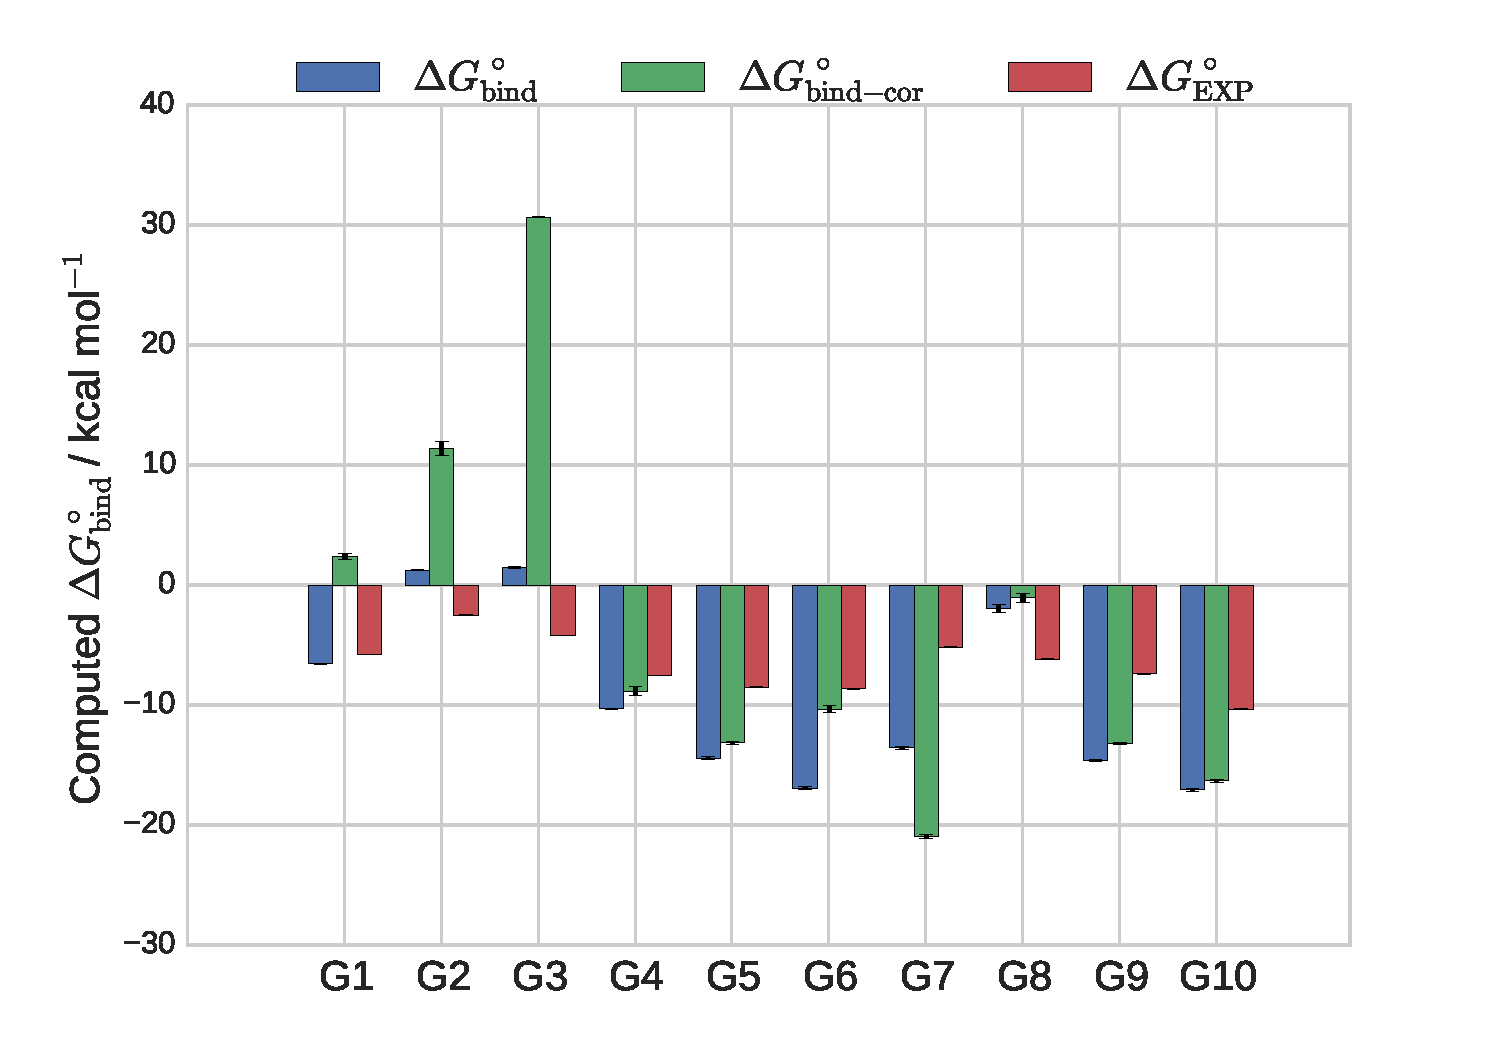
\includegraphics[width=\textwidth]{figures/Fig1.pdf}
 \centering
\end{figure}


\begin{table}[h!]
  \begin{minipage}{\linewidth}
  \caption{Details of charging free energy correction for ``SAMPL5 box'' protocol: $Q_\mathrm{L}$ is the solute charge in $e$, $\Delta G_\mathrm{bind}^\circ$ the standard free energy of binding, $\Delta G_\mathrm{COR}$ the charging free energy correction term evaluated with PB code, $\Delta G_\mathrm{bind--cor}^\circ$ the standard free energy of binding with charging correction, $\Delta G_\mathrm{EXP}$ the experimental binding free energy. All the values are expressed in kcal mol$^{-1}$ along with standard error of the mean (err)}\label{tab:tab1PBSAMPL5}
  \makebox[\textwidth][c]{
  \begin{tabular}{lccccccccc}
    \toprule
   molecule & $Q_\mathrm{L}$ & $\Delta G_\mathrm{bind}^\circ$ &err &$\Delta G^\mathrm{PBcode}_\mathrm{COR}$ & err & $\Delta G_\mathrm{bind-cor}^\circ$ & err  & $\Delta G_\mathrm{EXP}$ & err\\
    \midrule
G1 & 2 &-6.57 & 0.05 & 8.94 & 0.22 & 2.37 & 0.22 & -5.80 &0.03\\
G2 & 2 & 1.24 & 0.05 & 10.12& 0.57 & 11.36 & 0.57& -2.50 & 0.07\\
G3 & 4 & 1.46 & 0.09 & 29.18& 0.04 & 30.64 & 0.10& -4.02 & 0.03\\
G4 & 1 &-10.31& 0.06 & 1.47 & 0.38 & -8.84& 0.38 & -7.24 & 0.03\\
G5 & 1 &-14.43& 0.10 & 1.27 & 0.12 &-13.16& 0.16 & -8.53 & 0.07\\
G6 & 2 &-16.93& 0.13 & 6.58 & 0.24 &-10.34& 0.27 & -8.64 & 0.05\\
G7 &-2 &-13.55& 0.12 &-7.39 & 0.13 &-20.94& 0.17 & -5.17 & 0.02\\
G8 & 1 & -1.97& 0.35 & 0.88 & 0.09 & -1.08& 0.36 & -6.17 & 0.04\\
G9 & 1 &-14.91& 0.08 & 1.70 & 0.05 &-13.21& 0.10 & -7.40 & 0.02\\
G10& 1 &-17.07& 0.10 & 0.75 & 0.09 &-16.32& 0.14 & -10.35 & 0.02\\
  \bottomrule

 \end{tabular}
}
  \end{minipage}
\end{table}

Fig.~\ref{fig:fig1} and table~\ref{tab:tab1PBSAMPL5} report a comparison between the standard free energy of binding $\Delta G_\mathrm{bind}^\circ$, the standard free energy of binding after charging correction $\Delta G_\mathrm{bind-cor}^\circ$ and experimental values $\Delta G_\mathrm{EXP}$ for the host-guest system parametrized with the ``SAMPL5 box'' protocol ~\ref{sec:methods}.
$\Delta G_\mathrm{bind}^\circ$ are in line with experimental results with a $R^2$: 0.69< 0.70< 0.72 and MUE: 5.33< 5.40 < 5.47\SI{}{kcal mol^{-1}}. Large errors are present for guests G2 and G3, which are suppose to bind substantially worse than observed in experiments. Furthermore, these two molecules are made up of linear flexible alkyl chains and contain several positively charged ammonium groups.%By contrast, G4--G7, G9 and G10 are predicted to bind significantly better than experimentally observed. These compounds present a variety of net charges, but are all made up of conjugated aromatic rings. 
On the contrary, charging free corrections perform much worse with $R^2$: 0.07< 0.08 < 0.09 and MUE: 11.65< 11.79 < 11.94\SI{}{kcal mol^{-1}}. In particular, G2 and G3 show high positive free energy correction term $\Delta G_\mathrm{COR}$= \SI{10.12 +- 0.57}{kcal mol^{-1}} and \SI{29.18 +- 0.04}{kcal mol^{-1}} respectively. Additionally, negative charged molecules, as G7, has a more negative free energy correction term.
$\Delta G^\mathrm{PBcode}_\mathrm{COR}$=\SI{-7.39 +- 0.13}{kcal mol^{-1}}. Therefore, PBcode correction seems to be proportional to the solute charge: the higher charge the solute has the higher will be the $\Delta G_\mathrm{COR}$. 

Three main reasons can be drawn, to explain such a bias in the PB corrections:
\begin{itemize}
 \item First, the host is too flexible and theory~\ref{sec:pbcorrection} cannot work properly. Indeed, both ~\cite{Reif2014} and ~\cite{Rocklin} have shown very good results by measuring binding free energy only for large and rigid host molecules.
 \item Secondly, the force field parametrization may play a role, as found in ~\cite{LogD} with cyclohexane solvation free energies.
 \item Finally, the PB code may have some errors, especially in the Poisson-Boltzmann reaction field calculations.
\end{itemize}

In order to avoid possible box size effects which may influence the PB code itself, ``iso box'' protocol ~\ref{sec:methods} was applied to all the host-guest systems and charging free energy correction were re computed and fig. ~\ref{fig:fig2} and table~\ref{tab:tab2PBiso} show results. In this case, $\Delta G_\mathrm{bind}^\circ$ predictions show the same trend as before, with $R^2$=0.57 < 0.64< 0.70 and MUE = 4.85 < 5.10< 5.36 kcal mol$^{-1}$. On the other side, $\Delta G_\mathrm{bind--cor}^\circ$ has a better trend with respect to previous calculations, with an R$^2$= 0.39 < 0.41< 0.44 and MUE = 7.89< 8.14< 8.39 kcal mol$^{-1}$, although G2, G3 and G7 corrections are of the order of ten kcal mol$^{-1}$.
Higher standard error are present in these simulations, mainly due to the vanishing step in bound phase. Further tests will be done to assess the convergence of results between both kind of protocols.

\todo{This is very strange, SAMPL5 sire 15.1 HMR was more stable in boundphase vanishing step vs same box dim for hostguest sire 16.1 allbonds constraints }

\newpage
\begin{figure}[h!]
\caption{Comparison between standard free energy of binding $\Delta G_\mathrm{bind}^\circ$, standard free energy of binding after charging correction $\Delta G_\mathrm{bind-cor}^\circ$ and experimental binding free energy $\Delta G_\mathrm{EXP}$ using ``iso box'' protocol to prepare the free phase system \label{fig:fig2}}
 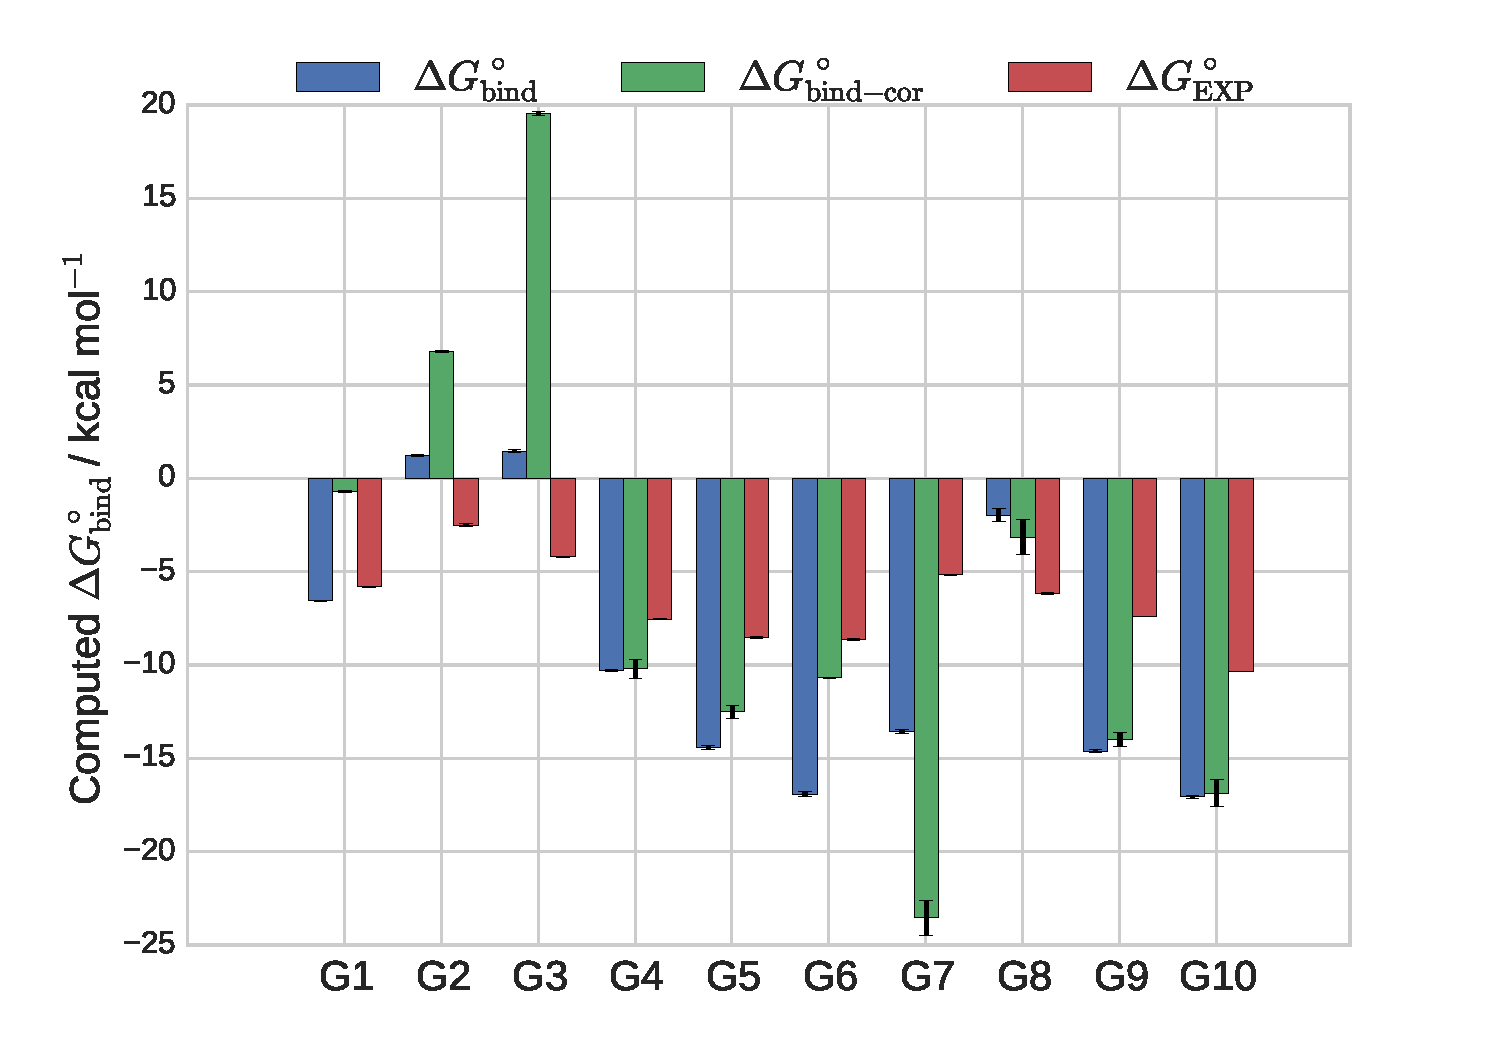
\includegraphics[width=\textwidth]{figures/Fig2.pdf}
 \centering
\end{figure}

\begin{table}[h!]
  \begin{minipage}{\linewidth}
  \caption{Details of charging free energy correction with ``iso box'' protocol: $Q_\mathrm{L}$ is the solute charge in $e$, $\Delta G_\mathrm{bind}^\circ$ the standard free energy of binding, $\Delta G_\mathrm{COR}$ the charging free energy correction term evaluated with PB code, $\Delta G_\mathrm{bind--cor}^\circ$ the standard free energy of binding with charging correction, $\Delta G_\mathrm{EXP}$ the experimental binding free energy. All the values are expressed in kcal mol$^{-1}$ along with standard error of the mean (err)}\label{tab:tab2PBiso}
  \makebox[\textwidth][c]{
  \begin{tabular}{lccccccccc}
    \toprule
   molecule & $Q_\mathrm{L}$ & $\Delta G_\mathrm{bind}^\circ$ &err &$\Delta G^\mathrm{PBcode}_\mathrm{COR}$ & err & $\Delta G_\mathrm{bind-cor}^\circ$ & err  & $\Delta G_\mathrm{EXP}$ & err\\
    \midrule
G1 & 2  & -8.52 & 0.02 & -0.71 & 0.04 &-5.80 &0.03\\
G2 & 2  & -1.93 & 0.12 &  6.79 & 0.05 &-2.50 & 0.07\\
G3 & 4  & -6.00 & 0.35 & 19.53 & 0.10 &-4.02 & 0.03\\
G4 & 1  &-11.28 & 0.59 & -10.21& 0.51 &-7.24 & 0.03\\
G5 & 1  & -13.77 & 0.13 & -12.51 & 0.33 & -8.53 & 0.07\\
G6 & 2  & -17.37& 0.07& -10.69& 0.02& -8.64 & 0.05\\
G7 &-2  & -15.45& 0.92& -23.54& 0.95&-5.17 & 0.02\\
G8 & 1  & -4.31 & 0.81 & -3.15& 0.93&-6.17 & 0.04\\
G9 & 1  & -15.45& 0.52 & -14.00& 0.38& -7.40 & 0.02\\
G10& 1  & -17.93 & 0.04 & -16.86& 0.07& -10.35 & 0.02\\
  \bottomrule

 \end{tabular}
}
  \end{minipage}
\end{table}

\newpage


\subsection{Thermodynamic cycle approach for charging free energy corrections}
\label{sec:tdbindingcharging}

 \todo{Fix results of SAMPL5box with SAMPL5 real results. Some of them are different since I did not add LJLRC, but why G8 is so different?}

\begin{figure}[h]
\caption{Comparison between standard free energy of binding $\Delta G_\mathrm{bind}^\circ$, standard free energy of binding after charging correction with thermodynamic cycle $\Delta G_\mathrm{bind-cor}^\circ$ ~\ref{sec:tdcorrection} and experimental binding free energy $\Delta G_\mathrm{EXP}$ with ``SAMPL5 box'' parametrization\label{fig:fig3}}
 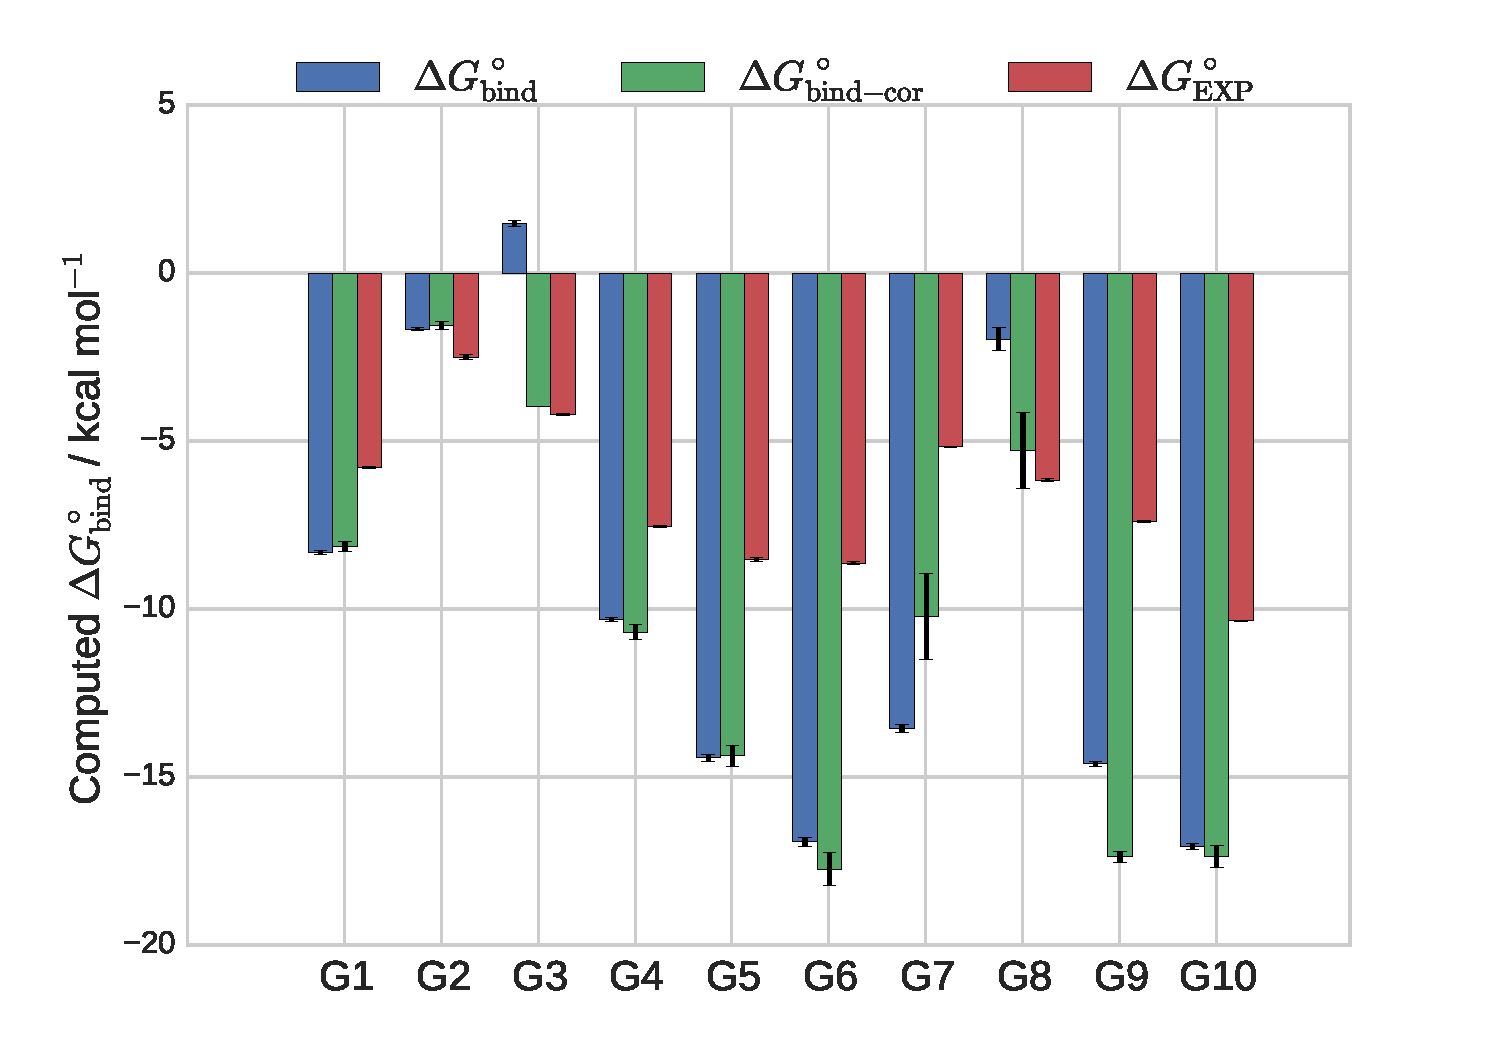
\includegraphics[width=\textwidth]{figures/Fig3.pdf}
 \centering
\end{figure}

\begin{table}[h!]
  \begin{minipage}{\linewidth}
  \caption{Standard free energy of binding $\Delta G_\mathrm{bind}^\circ$, charging free energy correction $\Delta G^\mathrm{TDion}_\mathrm{COR}$ evaluated with thermodynamic cycle ~\ref{sec:tdcorrection} and standard free energy of binding with charging correction $\Delta G_\mathrm{bind-cor}^\circ$ along with standard error (err)  for ``SAMPL5 box'' protocol } \label{tab:tab4TDSAMPL5}
  \makebox[\textwidth][c]{
  \begin{tabular}{lccccccccc}
    \toprule
   molecule & $Q_\mathrm{L}$ & $\Delta G_\mathrm{bind}^\circ$ &err &$\Delta G_\mathrm{COR}$ & err & $\Delta G_\mathrm{bind-cor}^\circ$ & err  & $\Delta G_\mathrm{EXP}$ & err\\
    \midrule
G1 & 2 &-8.32 & 0.05 & 0.18 & 0.22 & -8.14 & 0.14 & -5.80 &0.03\\
G2 & 2 &-1.67 & 0.05 & 0.10 & 0.15 & -1.57 & 0.12& -2.50 & 0.07\\
G3 & 4 & 1.34 & 0.09 &-5.31 & 0.01 & 30.64 & 0.10& -4.02 & 0.03\\
G4 & 1 &-10.21& 0.06 &-0.47 & 0.06 &-10.69 & 0.22& -7.24 & 0.03\\
G5 & 1 &-14.16& 0.32 &-0.21 & 0.02 &-14.37 & 0.32 & -8.53 & 0.07\\
G6 & 2 &-17.35& 0.26 &-0.39 & 0.23 &-17.74& 0.49 & -8.64 & 0.05\\
G7 &-2 &-12.46& 0.12 &-0.43 & 0.05 &-12.89& 1.27 & -5.17 & 0.02\\
G8 & 1 &-3.10 & 1.12 &-2.19 & 0.01 & -5.29& 1.13 & -6.17 & 0.04\\
G9 & 1 &-15.03& 0.08 &-2.34 & 0.08 &-17.37& 0.16 & -7.40 & 0.02\\
G10& 1 &-17.35& 0.21&-0.01 & 0.11 &-17.36& 0.33 & -10.35 & 0.02\\
  \bottomrule

 \end{tabular}
}
  \end{minipage}
\end{table}


Table ~\ref{tab:tab4TDSAMPL5} and fig~\ref{fig:fig3} show the standard free energy of binding $\Delta G_\mathrm{bind-cor}^\circ$ corrected with the thermodynamic approach depicted in fig XX, with host-guest systems parametrized with ``SAMPL5 box'' protocol.

In this case the final standard free energy of binding $\Delta G_\mathrm{bind-cor}^\circ$ presents a better trend with respect to experimental data, with an $R^2$: 0.65< 0.73< 0.79 and MUE of 4.47< 4.74< 5.04 kcal mol$^{-1}$.

Thus, to test the consistency of the thermodynamic cycle approach, all the CBC guests were solvated according to the ``iso box'' protocol and tab.~\ref{tab:tab5TDISOBOX} and fig.~\ref{fig:fig4} show the final estimations.
$\Delta G_\mathrm{bind-cor}^\circ$ is in line with results in tab.~\ref{tab:tab4TDSAMPL5} with an R$^2$=0.59< 0.66< 0.74 and MUE=4.43< 4.69< 4.96 kcal mol$^{-1}$. 
High standard errors are present, which are mainly due to fluctuations in the bound phase vanishing step, for molecule G4, G6, G7, G8 and G9. A further run will be made for these molecules to enhance convergence of results.
Overall, thermodynamic cycle approach seems to give a more reasonable charging correction, but a strict convergence of free energy changes is required to be more accurate and consistent.
\begin{table}[h!]
  \begin{minipage}{\linewidth}
  \caption{Details of charging free energy correction: $Q_\mathrm{L}$ is the solute charge in $e$, $\Delta G_\mathrm{bind}^\circ$ the standard free energy of binding, $\Delta G_\mathrm{COR}$ the charging free energy correction term, $\Delta G_\mathrm{bind-cor}^\circ$ the standard free energy of binding with charging correction, $\Delta G_\mathrm{EXP}$ the experimental binding free energy. All the values are expressed in kcal mol$^{-1}$ along with standard error (err)}\label{tab:tab5TDISOBOX}
  \makebox[\textwidth][c]{
  \begin{tabular}{lccccccccc}
    \toprule
   molecule & $Q_\mathrm{L}$ & $\Delta G_\mathrm{bind}^\circ$ &err &$\Delta G^\mathrm{TDion}_\mathrm{COR}$ & err & $\Delta G_\mathrm{bind-cor}^\circ$ & err  & $\Delta G_\mathrm{EXP}$ & err\\
    \midrule
G1 & 2 & -8.52& 0.02 & 0.53 & 0.06 & -7.98 & 0.03 & -5.80 &0.03\\
G2 & 2 & -1.93& 0.12 & 0.09 & 0.11 & -1.83 & 0.01 & -2.50 & 0.07\\
G3 & 4 & -6.00& 0.35 & 1.48 & 0.10 & -4.52 & 0.24 & -4.02 & 0.03\\
G4 & 1 &-11.28& 0.59 & 0.03 & 0.02 &-11.24 & 0.61 & -7.24 & 0.03\\
G5 & 1 &-13.77& 0.13 & 0.20 & 0.01 &-13.57 & 0.14 & -8.53 & 0.07\\
G6 & 2 &-17.37& 0.07 & 0.70 & 0.33 &-16.67 & 0.40 & -8.64 & 0.05\\
G7 &-2 &-15.45& 0.92 & 0.66 & 0.17 &-14.79 & 1.09 & -5.17 & 0.02\\
G8 & 1 & -4.31& 0.81 & 0.22 & 0.07 & -4.09 & 0.73 & -6.17 & 0.04\\
G9 & 1 &-15.45& 0.52 & 0.29 & 0.06 &-15.16 & 0.46 & -7.40 & 0.02\\
G10& 1 &-17.93& 0.04 & 0.35 & 0.09 &-17.57 & 0.05 & -10.35 & 0.02\\
  \bottomrule

 \end{tabular}
}
  \end{minipage}
\end{table}

\begin{figure}[h!]
\caption{Comparison between ``iso box'' standard free energy of binding $\Delta G_\mathrm{bind}^\circ$, standard free energy of binding after charging correction with thermodynamic cycle $\Delta G_\mathrm{bind-cor}^\circ$ ~\ref{sec:tdcorrection} and experimental binding free energy $\Delta G_\mathrm{EXP}$ \label{fig:fig4}}
 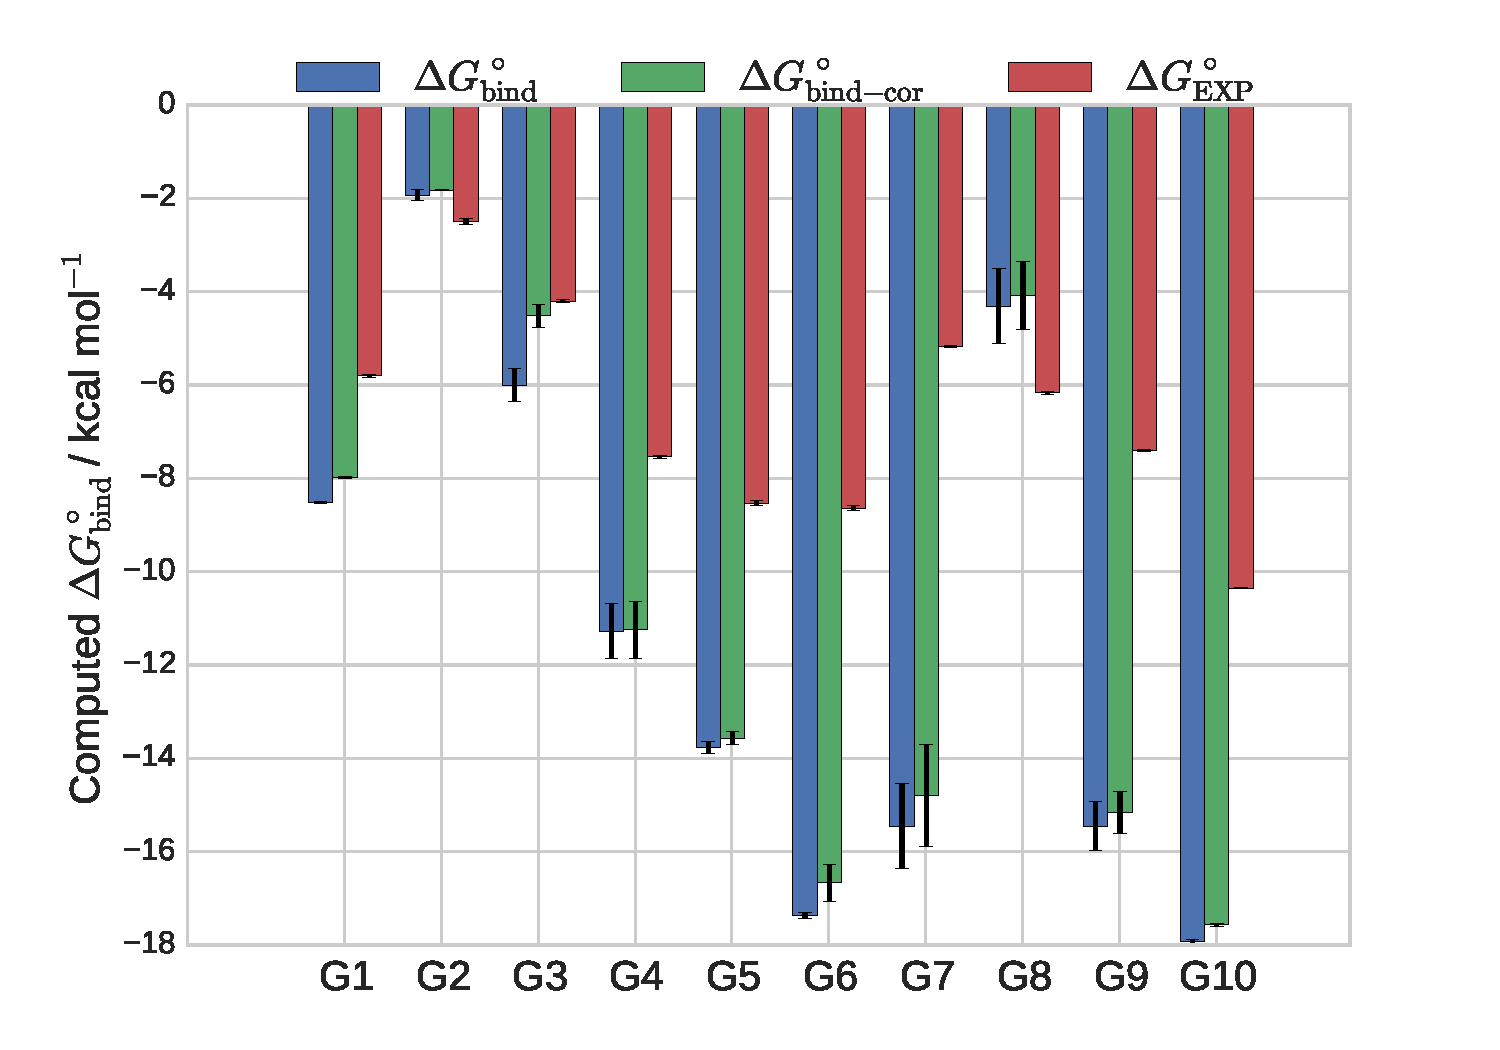
\includegraphics[width=\textwidth]{figures/Fig4.pdf}
 \centering
\end{figure}



\newpage

\bibliographystyle{unsrt}
\bibliography{charge}{}



\end{document}
